
\section{固溶时效处理的强化作用研究}
在本设计有限的实验基础上,为了能深入研究固溶时效对于\ti 合金的强化作用,进一步确定最佳的热处理工艺,笔者统计了近年来的相关的一些研究报告,得到了如\ref{sec:mytcstrengthave}的数据:
\begin{table}[htbp]
	\centering
			\zihao{5}
	\caption{不同实验所得的TC4强度统计}
	\label{sec:mytcstrengthave}
	\begin{tabular}{cccc}
		\toprule
		类型& $ \sigma_{0.2} $屈服强度/MPa  &$ \sigma_m $抗拉强度/MPa &延伸率$ \delta \% $ \\ \midrule
		平均值 & 953.541& 1001.874&12.160 \\
		方差 &97.116& 105.897& 4.077 \\
		标准差 &9656.014&11438.403&16.952 \\
		最大值 &  1110 & 1218 & 19 \\
		最小值&700 & 790 & 3.78 \\
		极差&410 & 428 & 15.22 \\
		\bottomrule
	\end{tabular}
\end{table}


从强度上来看,大多数试样的原始抗拉强度都在850MPa以上,屈服强度在830MPa以上,基本满足国家标准\ref{sec:mytc4machins}的要求。试样在经过固溶、时效等热处理方式处理过后,抗拉强度与屈服强度平均增加了200MPa左右,分别达到了900MPa与1200MPa之间。其中,最高的强度是鲁媛媛等\cite{luyuanyuanShixiaochuliduiTC4taihejinweiguanzuzhihelixuexingnengdeyingxiang2019}在970℃$ \beta $相变点附近进行固溶处理后,再通过550℃/300min(AC)方式下得到的组织,其抗拉强度$ \sigma_m $达到了1218MPa,屈服强度%\footnote{标准术语为“塑性延伸强度”,当塑性延伸率为$0.2\%  $时即为屈服强度}
为$ \sigma_{0.2} $为1109MPa,可见热处理对于组织的优化还是很可观的。
\begin{table}[htbp]
	\centering
			\zihao{5}
	\caption{TC4合金力学性能的国家标准}
	\label{sec:mytc4machins}
	\begin{tabular}{cccc}
		\toprule
		力学性能& 抗拉强度$MPa  $& 屈服强度$ MPa $&断后伸长率$ \% $\\ \midrule
		标准值 &$ \ge 895 $&$ \ge 830 $&$ \ge 10 $ \\ \bottomrule
	\end{tabular}
\end{table}


在不同固溶温度的处理下,可以得到不同的组织,进而呈现出不同的力学性能。如\ref{fig:固溶温度与强度}所示,通过分析可得:研究者集中在900℃到1000℃之间进行固溶处理,且在温度达到960℃附近的时候,合金拥有相对较大的屈服强度与抗拉强度。
\begin{figure}[h!]
	\centering
	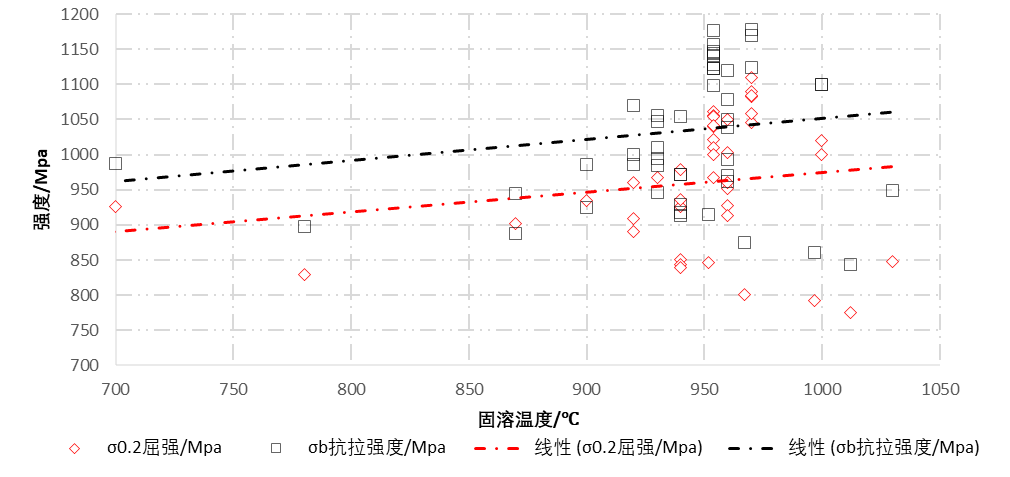
\includegraphics[width=0.7\linewidth]{TC4钛合金热处理研究进展/固溶温度与强度}
	\caption{固溶温度与强度}
	\label{fig:固溶温度与强度}
\end{figure}

如\ref{fig:时效温度与抗拉屈服强度}所示,通过分析可得,研究者集中在500℃与725℃附近,而在550℃左右时进行时效处理得到的合金强度较大。
\begin{figure}[h!]
	\centering
	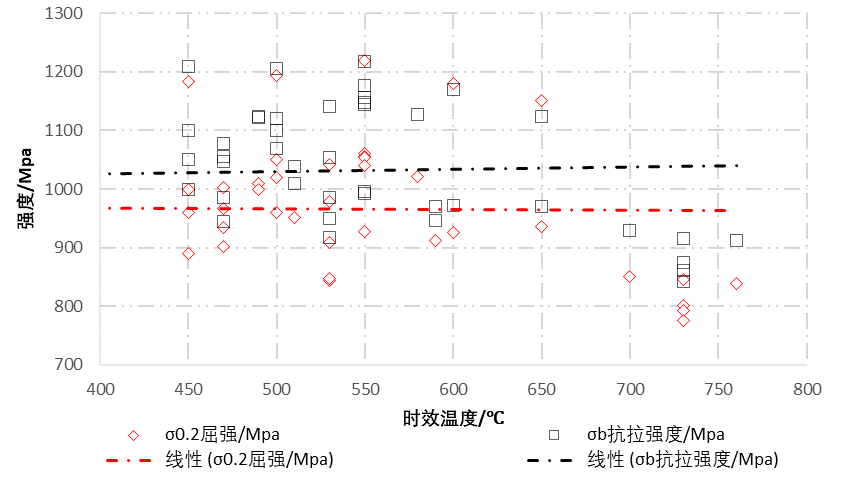
\includegraphics[width=0.7\linewidth]{TC4钛合金热处理研究进展/时效温度与强度}
	\caption{时效温度与抗拉屈服强度}
	\label{fig:时效温度与抗拉屈服强度}
\end{figure}

\begin{figure}[h!]
	\centering
	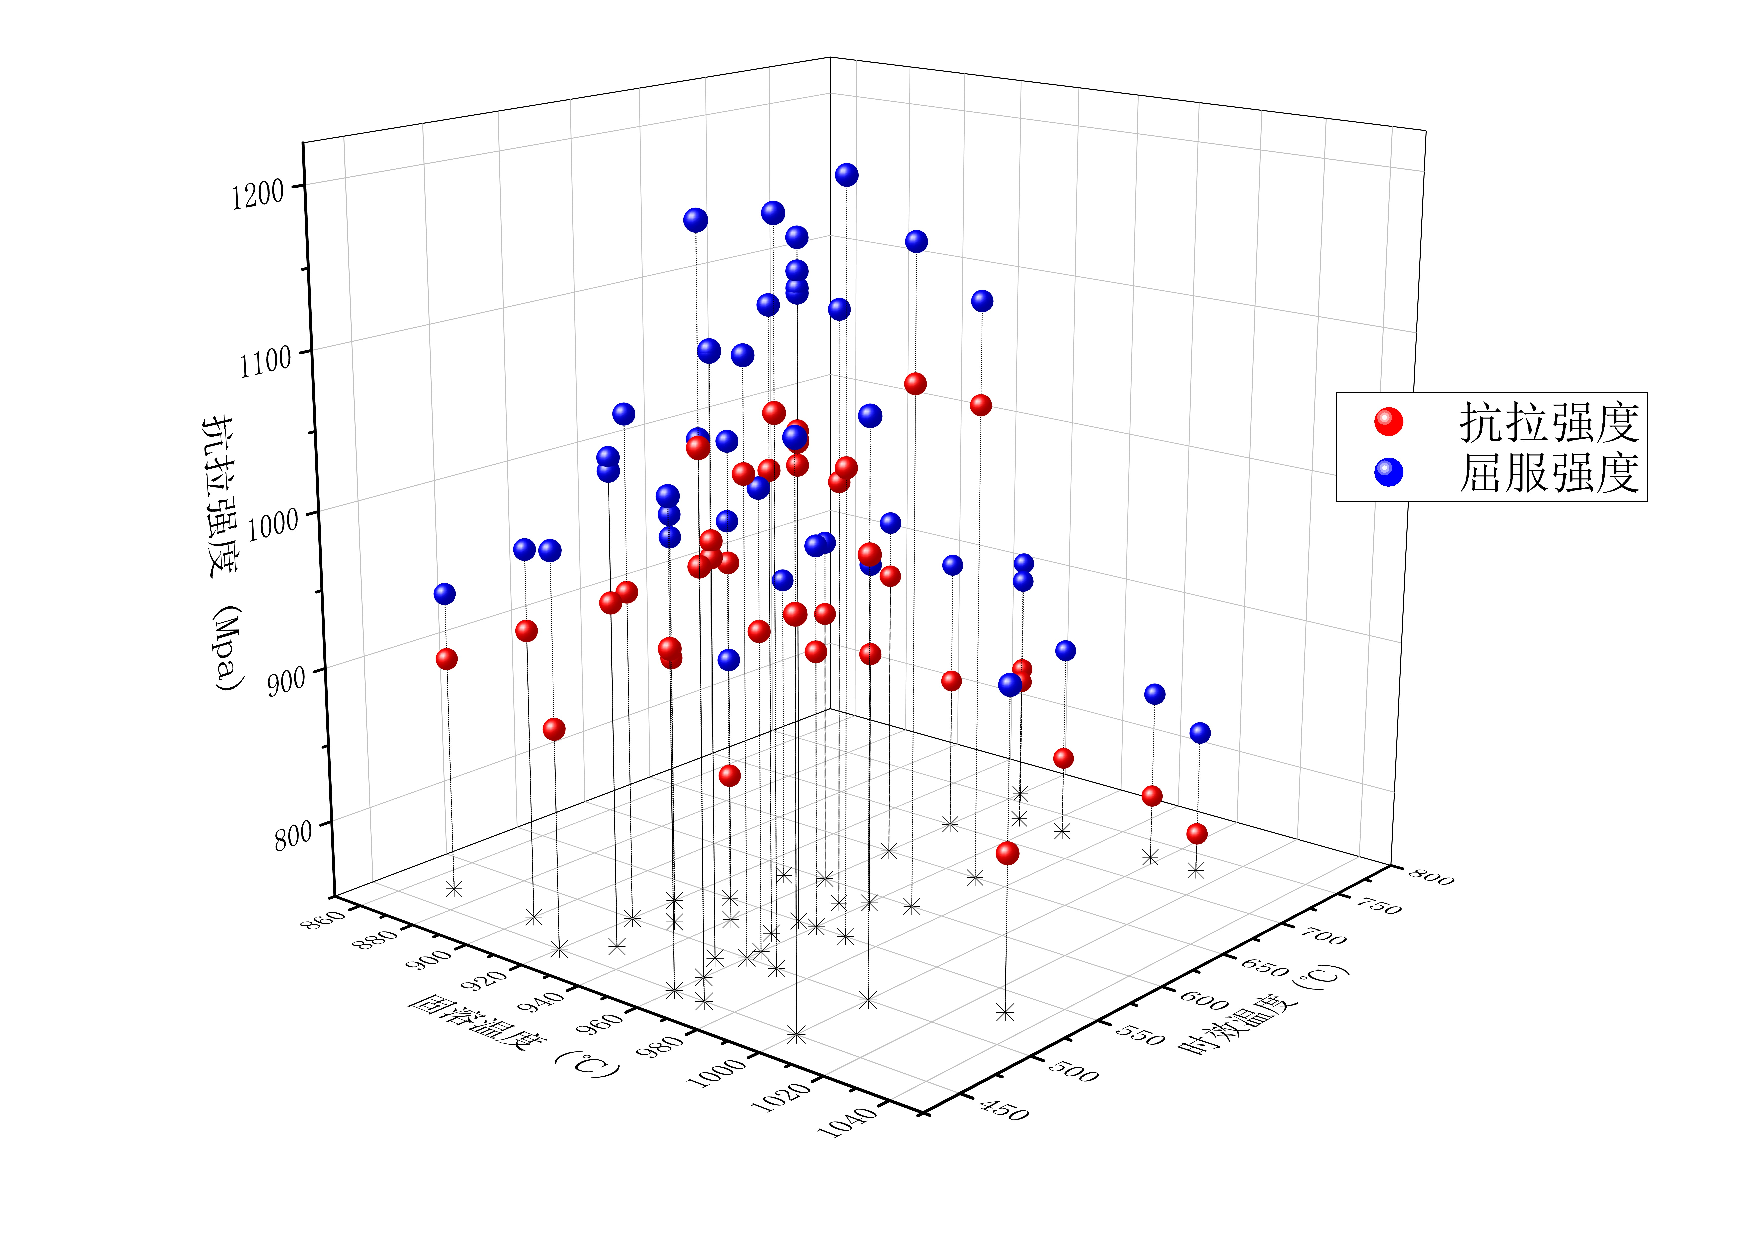
\includegraphics[width=0.7\linewidth]{TC4钛合金热处理研究进展/固溶温度、时效温度与强度}
	\caption{固溶温度、时效温度与强度三维图}
	\label{fig:}
\end{figure}
综上分析,当固溶温度选择在960℃附近、时效温度选择在550℃附近时可以得到较好的力学性能,这与本设计的实验结果是一致的。

